\section{Modeling Process}
\label{sec:modeling} 

%\textcolor{red}{Decision Tree}

For Yelp rating prediction, we use Decision Tree, which is tree-like graph of decisions and their possible consequences. It is widely used prediction model in machine learning. In this tree structure, leaves represent class labels and branches represent conjunctions of features that lead to the class labels. A typical example is shown in Figure \ref{fig:DT} \footnote{\url{https://en.wikipedia.org/wiki/Decision_tree_learning}}. The modeling process include feature selection, best split, feature ranking and tree generation. 

%-------------------------------------------
\begin{figure}[h]
	\centering
	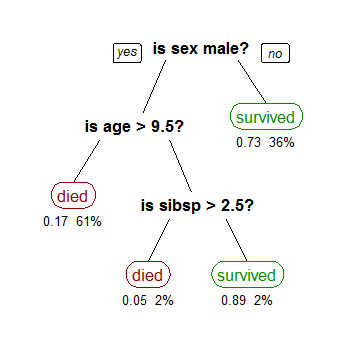
\includegraphics[width=5cm]{DT.png}
	\caption{A Decision Tree showing survivals of passengers of the Titanic.}
	\label{fig:DT}
\end{figure}
%------------------------------------------- 

\paragraph{Feature Selection}
%There are multiple features related a user's rating. \textcolor{red}{give list or table, showing all features. }
Yelp dataset contains 11 tables such as Yelp dataset contains 11 tables such as business, category, checkin, etc. Figure \ref{fig:data}\footnote{\url{https://www.yelp.com/dataset/documentation/sql}} shows the dataset structure. We extract 22 features(shown in Table \ref{tb:feature}, which could be divided into four groups: user-related features(7), business-related features(3), user-category features(5) and review-related features(7).

%-------------------------------------------
\begin{figure}[h]
	\centering
	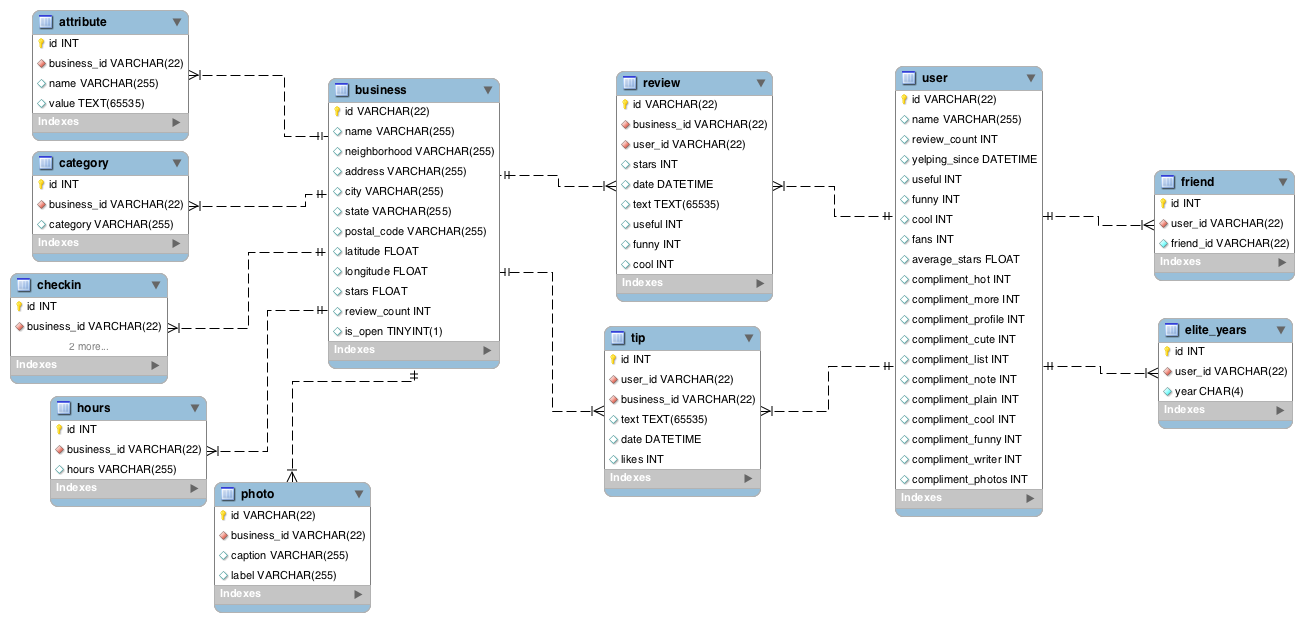
\includegraphics[width=6cm]{data.png}
	\caption{The structure of Yelp Dataset}
	\label{fig:data}
\end{figure}
%------------------------------------------- 
\newcommand{\tabincell}[2]{\begin{tabular}{@{}#1@{}}#2\end{tabular}}
\begin{table}
\centering
\caption{Feature Groups}
\label{table:para_regression}
\begin{tabular}{|c|c|}
\hline
Feature Group & Features \\ \hline
User-related Features(7) & \tabincell{c}{user compliment count\\user funny count\\user cool count\\user useful count\\user fans count \\ user review count \\ user average rating} \\ \hline
Business-related Features(3) & \tabincell{c}{business average rating\\business location-related rating\\business neighborhood-related rating} \\ \hline
Review-related Features(7) & \tabincell{c}{Polarity \\  Subjectivity  \\  TF-IDF  \\ Meaningful word count  \\ review useful count\\ review cool count \\ review funny count  } \\  \hline
User-category Features(5) & \tabincell{c}{  uc-review count   \\  uc-average rating  \\ uc-review funny count \\  uc-review  cool count   \\  uc-review useful count }\\
\hline
\end{tabular}
\end{table}


\paragraph{Best Split}
Decision Tree works in a top-down manner, we need to choose a variable at each step that best split the sets of items. The best split are chosen by certain metric, e.g., Gini impurity, Information gain and so on. 

\paragraph{Feature Ranking}
Feature ranking helps us have a better understanding of how each feature contribute to our model training. Table \ref{tb:ranking} shows the result of our 22 feature ranking. From this table we can know that review's polarity, user to a certain category's average rating, user to a certain category's review count.

\begin{table}[h]
	\small
	\caption{Feature Ranking Results}
	\label{tb:ranking}
	\begin{tabular}{l|l}
		\hline
		\textbf{Feature}                          & \textbf{F score (scaled)}                                                                \\ \hline
		polarity     & 85                       \\ \hline
		uc-average rating      & 67                        \\ \hline
		uc-review count & 42\\ \hline
		subjectivity & 42\\ \hline
		business average rating & 29\\ \hline
		user average rating & 26\\ \hline
		user useful count & 16\\ \hline
		review useful count     & 16                       \\ \hline
		TF-IDF      & 16                        \\ \hline
		user review count & 16\\ \hline
		user compliment count & 14\\ \hline
		review cool count & 11\\ \hline
		review funny count & 10\\ \hline
		uc-review useful count& 8\\ \hline
		user funny count & 8\\ \hline
		user fans count     & 6                       \\ \hline
		user cool count      & 4                        \\ \hline
		uc-review cool count & 2\\ \hline
		uc-review funny count & 1\\ \hline
		business location-related rating & 1\\ \hline
		business neighborhood-related rating & 1\\ \hline
		meaningful word count& 1\\

	\end{tabular}
\end{table}

\paragraph{Tree Generation}
With the selected features, and variables chosen by best split, a tree can be generated. And each path in the tree represents a decision-making process, in which a user's rating can be predicted based on a series of decision makings. Here we use only 80 users to train our model. Under this situation, even though the generated decision tree has really simple structure and only top three features are involved, the trained model could still have high prediction accuracy(100\%).